\documentclass[tikz,border=10pt]{standalone}
\usepackage{tikz}
\usepackage{amsmath}
\usetikzlibrary{arrows.meta,positioning}

\begin{document}
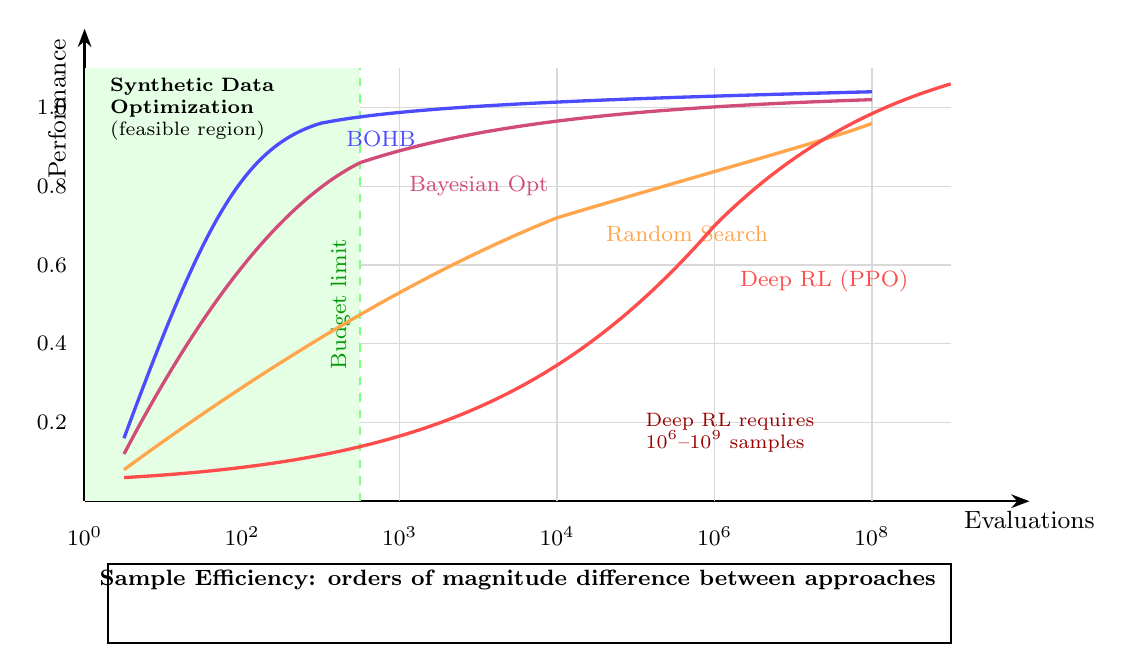
\begin{tikzpicture}[
    scale=1.0,
    every node/.style={font=\small}
]

% Axes
\draw[-{Stealth}, thick] (0,0) -- (12,0) node[anchor=north, font=\small] {Evaluations};
\draw[-{Stealth}, thick] (0,0) -- (0,6) node[anchor=east, font=\small, rotate=90, yshift=10pt] {Performance};

% X-axis labels (log scale)
\node[anchor=north, font=\footnotesize] at (0,-0.2) {$10^0$};
\node[anchor=north, font=\footnotesize] at (2,-0.2) {$10^2$};
\node[anchor=north, font=\footnotesize] at (4,-0.2) {$10^3$};
\node[anchor=north, font=\footnotesize] at (6,-0.2) {$10^4$};
\node[anchor=north, font=\footnotesize] at (8,-0.2) {$10^6$};
\node[anchor=north, font=\footnotesize] at (10,-0.2) {$10^8$};

% Y-axis labels
\node[anchor=east, font=\footnotesize] at (-0.1,1) {0.2};
\node[anchor=east, font=\footnotesize] at (-0.1,2) {0.4};
\node[anchor=east, font=\footnotesize] at (-0.1,3) {0.6};
\node[anchor=east, font=\footnotesize] at (-0.1,4) {0.8};
\node[anchor=east, font=\footnotesize] at (-0.1,5) {1.0};

% Grid lines
\foreach \x in {2,4,6,8,10} {
    \draw[gray!30, thin] (\x,0) -- (\x,5.5);
}
\foreach \y in {1,2,3,4,5} {
    \draw[gray!30, thin] (0,\y) -- (11,\y);
}

% Feasible region shading
\fill[green!10] (0,0) rectangle (3.5,5.5);
\draw[green!50, dashed, thick] (3.5,0) -- (3.5,5.5);
\node[anchor=south, font=\footnotesize, green!60!black, rotate=90] at (3.5,2.5) {Budget limit};

% BOHB/Multi-fidelity curve (best - reaches high performance quickly)
\draw[blue!70, very thick]
    (0.5, 0.8) .. controls (1.5, 3.5) and (2, 4.5) .. (3, 4.8)
    .. controls (4, 5) and (6, 5.1) .. (10, 5.2);
\node[blue!70, anchor=west, font=\footnotesize] at (3.2, 4.6) {BOHB};

% Bayesian Optimization curve (good but slower)
\draw[purple!70, very thick]
    (0.5, 0.6) .. controls (1.5, 2.5) and (2.5, 3.8) .. (3.5, 4.3)
    .. controls (5, 4.8) and (7, 5) .. (10, 5.1);
\node[purple!70, anchor=west, font=\footnotesize] at (4, 4.0) {Bayesian Opt};

% Random Search curve (baseline)
\draw[orange!70, very thick]
    (0.5, 0.4) .. controls (2, 1.5) and (4, 2.8) .. (6, 3.6)
    .. controls (8, 4.2) and (9.5, 4.6) .. (10, 4.8);
\node[orange!70, anchor=west, font=\footnotesize] at (6.5, 3.4) {Random Search};

% Deep RL curve (needs many samples)
\draw[red!70, very thick]
    (0.5, 0.3) .. controls (4, 0.5) and (6, 1.2) .. (8, 3.5)
    .. controls (9, 4.5) and (10, 5) .. (11, 5.3);
\node[red!70, anchor=west, font=\footnotesize] at (8.2, 2.8) {Deep RL (PPO)};

% Annotations
\node[anchor=north west, text width=3cm, font=\scriptsize, align=left] at (0.2, 5.5)
    {\textbf{Synthetic Data}\\\textbf{Optimization}\\(feasible region)};

\node[anchor=south west, text width=2.5cm, font=\scriptsize, align=left, red!60!black] at (7, 0.5)
    {Deep RL requires\\$10^6$--$10^9$ samples};

% Legend box
\draw[thick] (0.3, -1.8) rectangle (11, -0.8);
\node[font=\footnotesize\bfseries] at (5.5, -1) {Sample Efficiency: orders of magnitude difference between approaches};

\end{tikzpicture}
\end{document}
